\documentclass{article}
\usepackage{amsmath,amsfonts,amsthm,amssymb}
\usepackage{setspace}
\usepackage{fancyhdr}
\usepackage{lastpage}
% \usepackage{extramarks}
% \usepackage{chngpage}
\usepackage[noabbrev]{cleveref}
\usepackage{soul,xcolor}
\usepackage{graphicx,float,wrapfig}
% \usepackage{CJK}
\usepackage{url}
\usepackage{algorithm}
\usepackage{algorithmicx}
\usepackage{algpseudocode}
\usepackage{enumitem}
% \usepackage{tikz}
% \usepackage{authblk}
\usepackage{listings} 
\newcommand{\Class}{Operating Systems and Distributed Systems}
\newcommand{\ClassInstructor}{Wei Xu}

% Homework Specific Information. Change it to your own
\newcommand{\Title}{Project 2 - SophiaCoin}
\newcommand{\DueDate}{Jan 20, 2024}

% In case you need to adjust margins:
\topmargin=-0.45in      %
\evensidemargin=0in     %
\oddsidemargin=0in      %
\textwidth=6.5in        %
\textheight=9.0in       %
\headsep=0.25in         %

% Setup the header and footer
\pagestyle{fancy}                                                 %
\chead{\Title}  %                                                  %
\cfoot{}                                                                %
\rfoot{Page\ \thepage\ of\ \protect\pageref{LastPage}}                  %
\renewcommand\headrulewidth{0.4pt}                                      %
\renewcommand\footrulewidth{0.4pt}                                      %

%%%%%%%%%%%%%%%%%%%%%%%%%%%%%%%%%%%%%%%%%%%%%%%%%%%%%%%%%%%%%
% Make title
\title{\textmd{\bf \Title}\\{\large Instructed by \textit{\ClassInstructor}}\\\normalsize\vspace{0.1in}\small{Due\ on\ \DueDate}}
\date{}
\newcommand*{\affaddr}[1]{#1} % No op here. Customize it for different styles.
\newcommand*{\affmark}[1][*]{\textsuperscript{#1}}
\newcommand*{\email}[1]{\texttt{#1}}

\author{%
Fangyan Shi\affmark[1], Chengda Lu\affmark[2], and Yiying Wang\affmark[3]\\
\affaddr{\affmark[1]2021010892 \affmark[2]2021010899 \affmark[3]2020011604}\\
\email{\{\affmark[1]sfy21,\affmark[2]lucd21,\affmark[3]wangyiyi20\}@mails.tsinghua.edu.cn}\\
}
 
%%%%%%%%%%%%%%%%%%%%%%%%%%%%%%%%%%%%%%%%%%%%%%%%%%%%%%%%%%%%%

\begin{document}
\begin{spacing}{1.1}
\maketitle \thispagestyle{empty}
%\cite{}
%%%%%%%%%%%%%%%%%%%%%%%%%%%%%%%%%%%%%%%%%%%%%%%%%%%%%%%%%%%%%
% Begin edit from here

\newcommand{\bb}[1]{\mathbf{#1}}
\newcommand{\FIGDIR}{/home/osgroup4/Documents/os-project/temp/fig} % This is to be filled by makefile

\section{Project Introduction}
In this project, we designed a decentralized transaction system called SophiaCoin. The transaction system imitates that of Bitcoin \cite{bitcoin}, but for simplification, the system uses pure public key as the address and supports only basic transactions, without an implementation for contracts. 

In this report, we will introduce how we design the block chain system, how we implemented the miner and the client, and a brief explanation of how they will be working correctly. For the fluency of whole report, we'll \textcolor{red}{NOT} introduce the optimizations (as a requirement for part II) individually in a section. They will be clearly mentioned as we illustrate the implementation.

\section{Data Structure and Consensus Rules}

In this section, we will introduce the data structure of our block chain and the block validation rules, or consensus rules. This section will adopt a top-down manner to illustrate every single detail.

First let's take a took at chain and blocks. See the following \cref{fig:chain}. Each block is composed by four fields: timestamp, nonce, the hash pointer to the previous block and the merkle root of transactions recorded by the block. Notice that each block has a hash pointer to the previous block, so all blocks will form a chain structure. The consensus rule will focus on the genesis block. We defined the genesis block as shown in \cref{fig:chain}, with each field fixed in hard code. Therefore, the first block must have a fixed pointer. The consensus rules also require that the block hash must satisfy the classical proof-of-work criterion, which is well-known.

\begin{figure}[htbp]
    \centering
    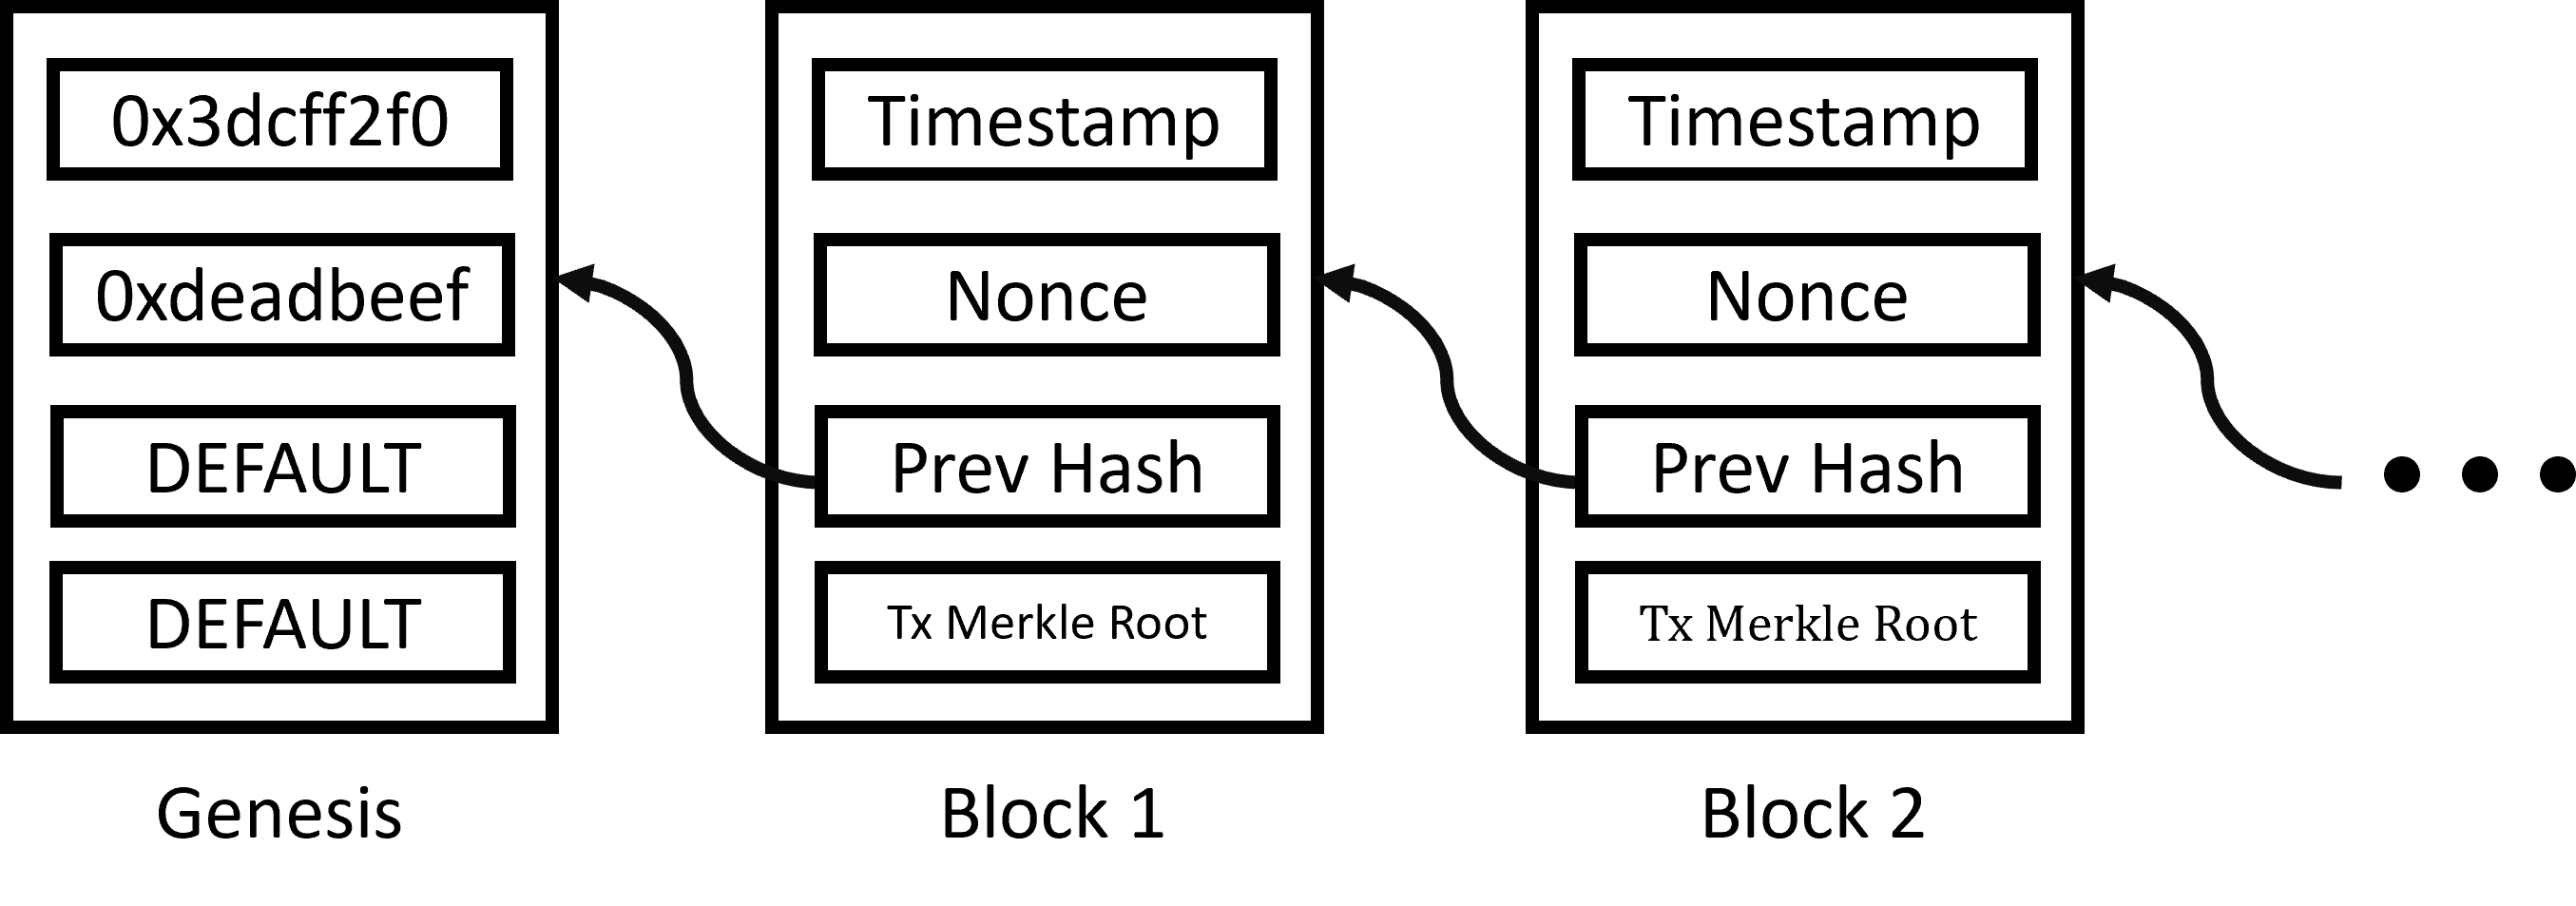
\includegraphics[width=.6\linewidth]{\FIGDIR/chain.png}
    \caption{Chain of Blocks}
    \label{fig:chain}
\end{figure}

Second, we focus on how transactions are stored in a block. The data structure we adopt is merkle tree, which is \textcolor{red}{THE FIRST OPTIMIZATION}. We show the case of 5 transactions(including the coinbase construction) in \cref{fig:merkle}. The consensus rule requires that the merkle root of the merkle tree shall match the fourth field in a block. Only with this optimization can we better design our lightweight client, which will be introduced later.

\begin{figure}[htbp]
    \centering
    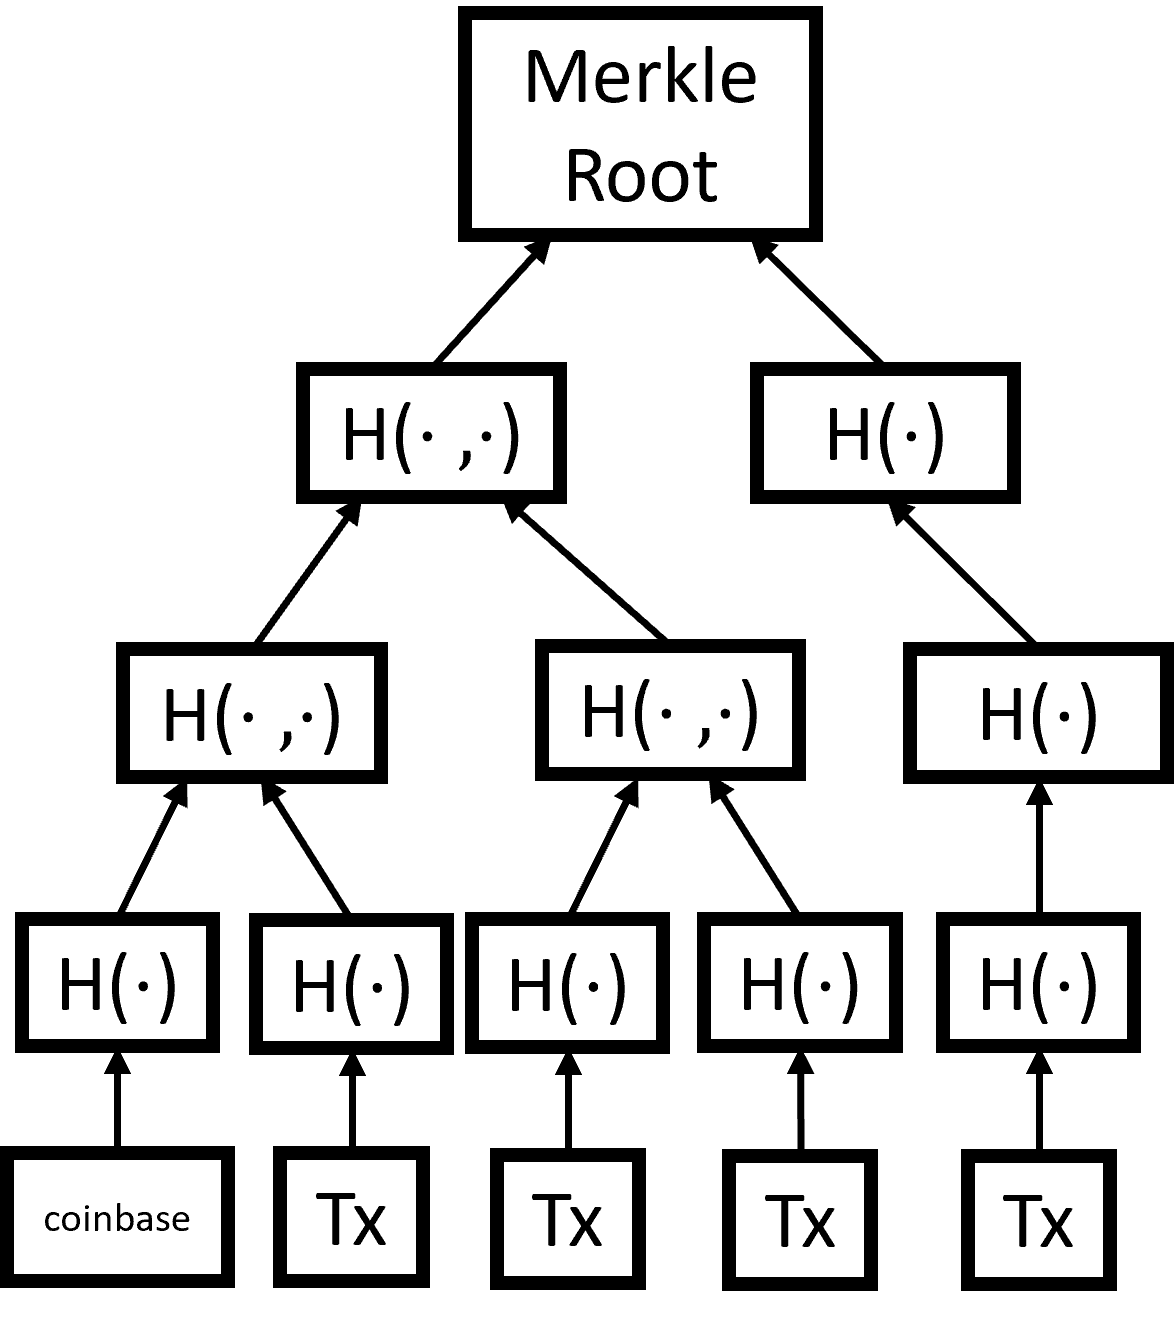
\includegraphics[width=.4\linewidth]{\FIGDIR/merkle.png}
    \caption{Merkle Tree}
    \label{fig:merkle}
\end{figure}

Finally, let's take a look at the structure of transactions. Transaction structure is indicated by \cref{fig:transaction}. Notice that each transaction is composed by TxIn, TxOut and signatures. TxIn is composed by a hash pointer to a transaction and an integer, which servers as a pointer to a transaction out. TxOut is composed by a public key and an integer, indicating the payment address and how many coins are transferred. Signatures are just a sequence of bytes.
\begin{figure}[htbp]
    \centering
    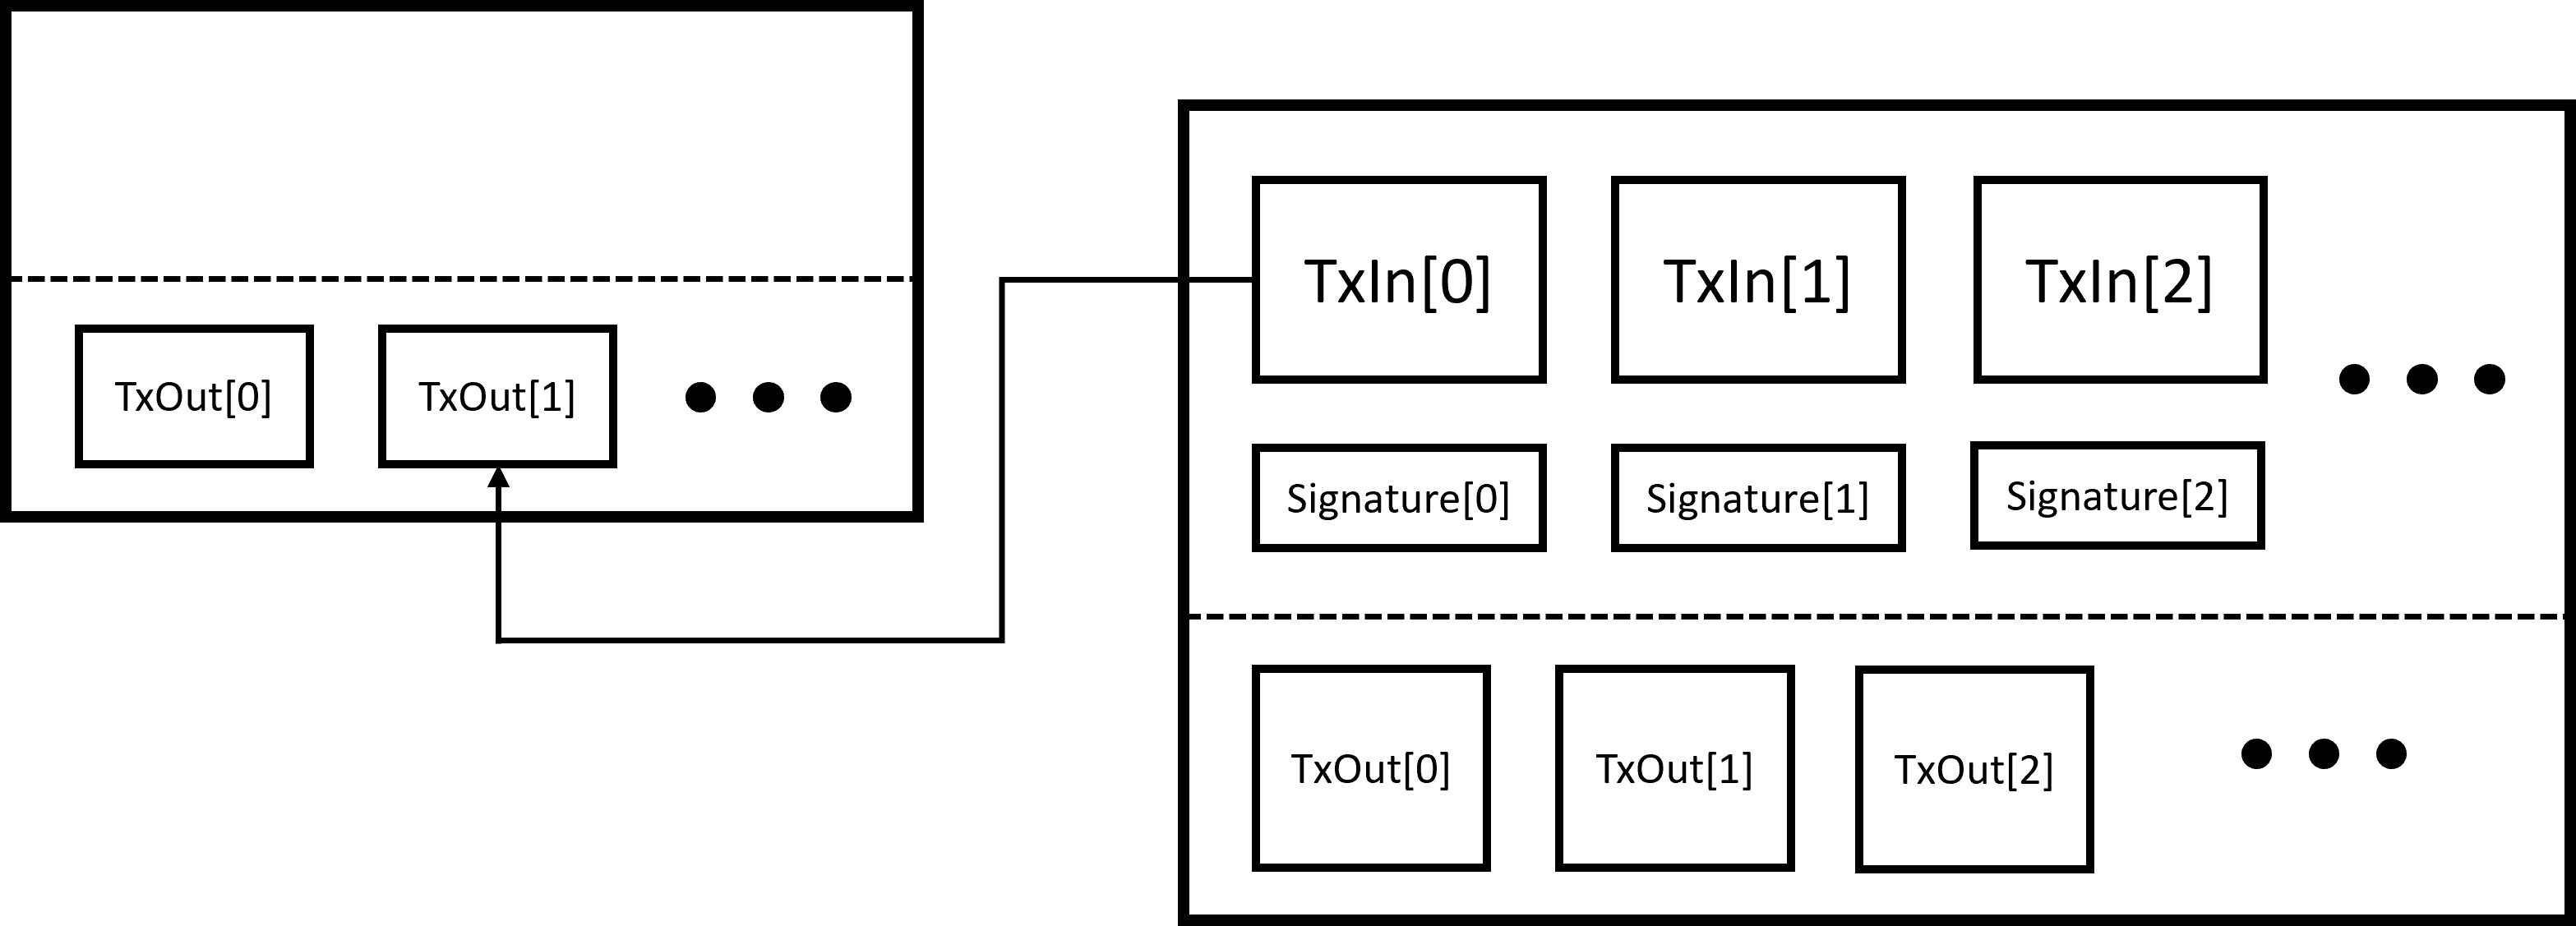
\includegraphics[width=.7\linewidth]{\FIGDIR/transaction.png}
    \caption{Transaction}
    \label{fig:transaction}
\end{figure}

Notice in \cref{fig:merkle}, there are normal transactions and a coinbase transaction in a block. For normal transactions, the consensus rules require that 
\begin{itemize}
    \setlength\itemsep{1pt}
    \item The number of signatures is the same with number of TxIns. Therefore, each signature serves the TxIn with the same index.
    \item Each signature must be signed by the public key of the TxOut pointed by the corresponding TxIn.
    \item The total amount of TxOuts is no larger than the total amount of TxOuts pointed by the TxIns(The remaining amount is served as tips).
\end{itemize}

For a coinbase transaction, we have the following structure as shown in \cref{fig:coinbase}. We requires that there are only one TxIn and no signatures. The TxIn must have a default hash pointer and the index shall be the block height. The total amount of TxOuts shall be equal to \textbf{1024} plus total tips of all normal transactions at the specific block. Therefore, 1024 coins are minted as a miner creates a new block.

\begin{figure}[htbp]
    \centering
    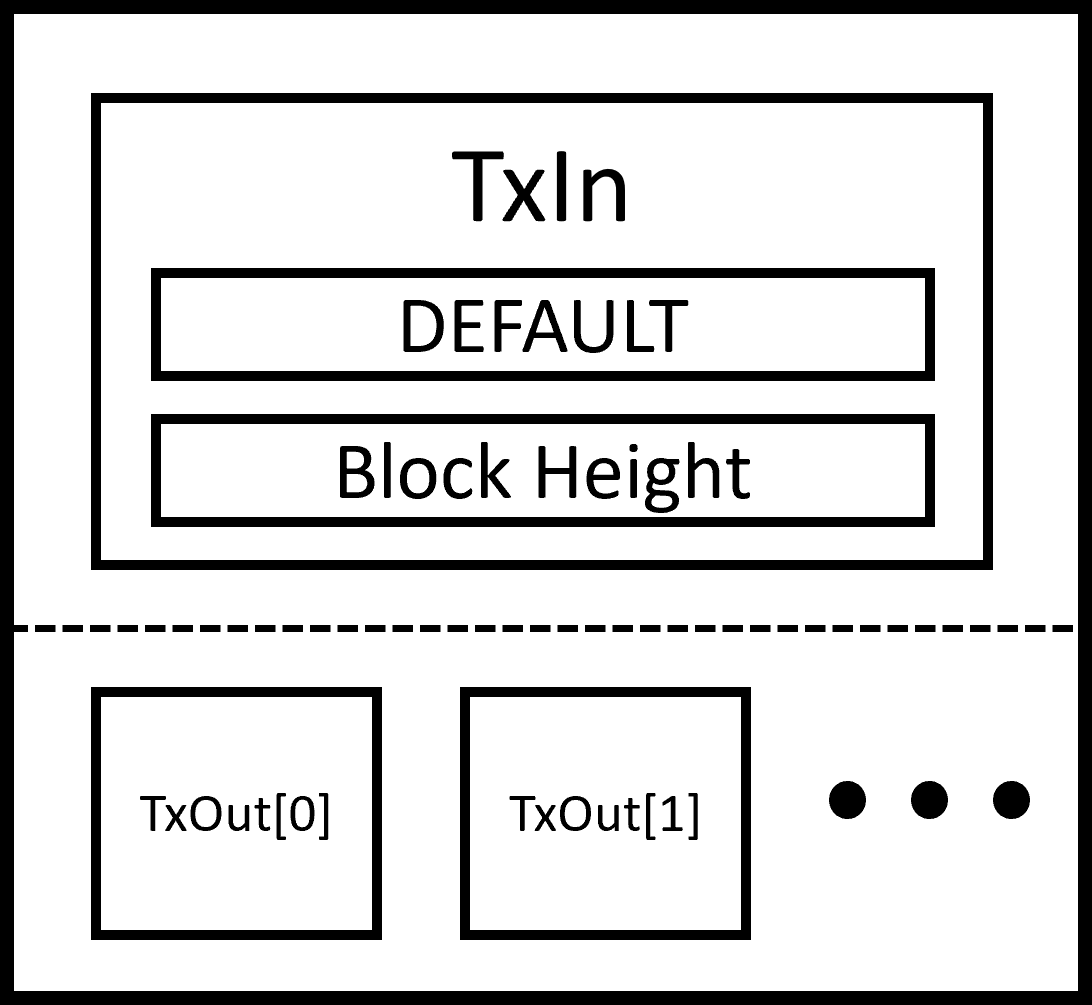
\includegraphics[width=.3\linewidth]{\FIGDIR/coinbase.png}
    \caption{Coinbase Transaction}
    \label{fig:coinbase}
\end{figure}

\section{How Miners Work?}

In this section, we'll introduce the implementation details of the miner process. We illustrate the miner process in \cref{fig:miner}, which give a full view of how a miner works. Each part will be elaborated in the following subsections.

\begin{figure}[htbp]
    \centering
    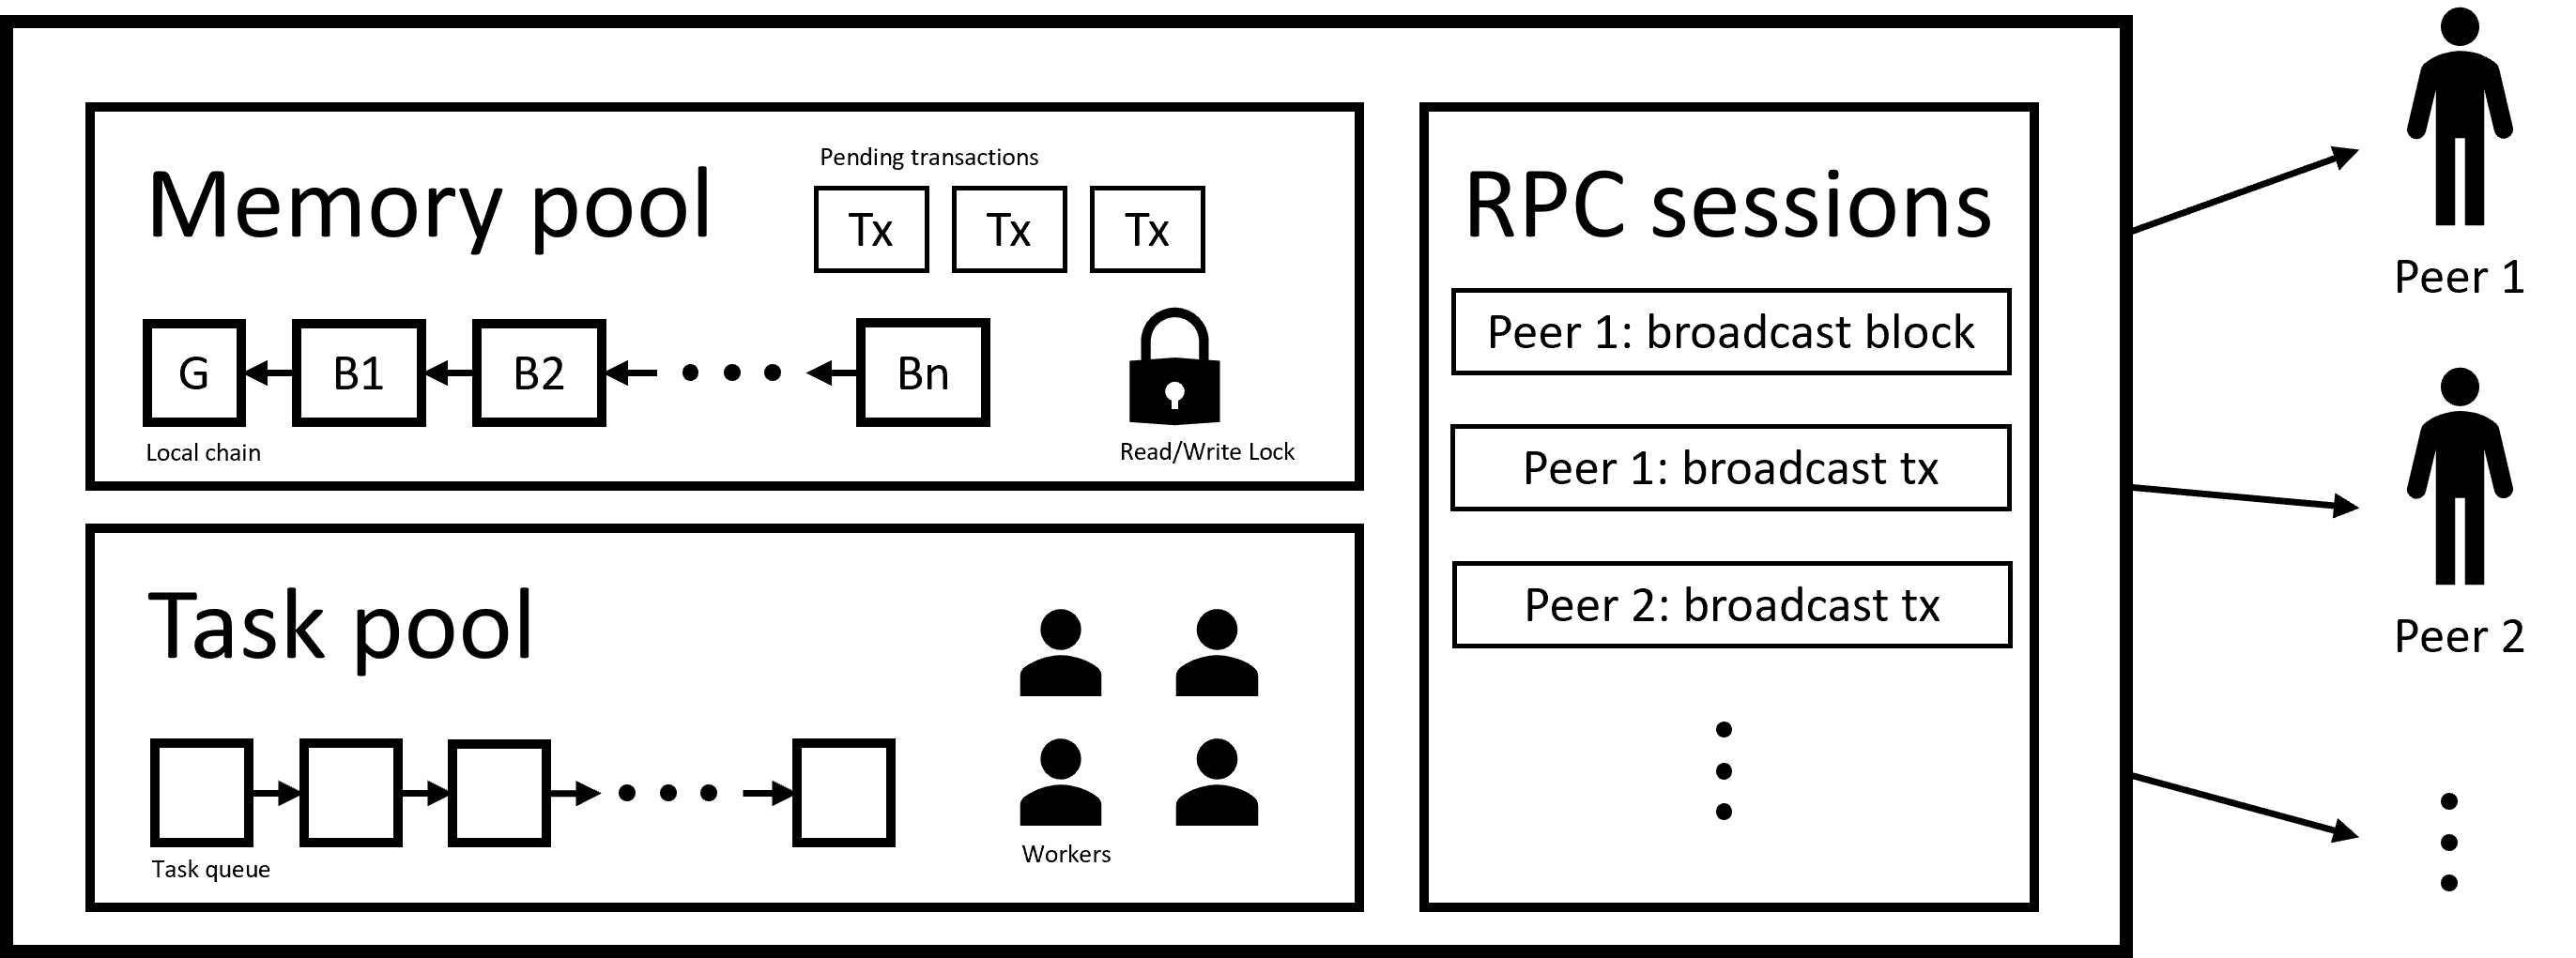
\includegraphics[width=.8\linewidth]{\FIGDIR/miner.png}
    \caption{Miner process}
    \label{fig:miner}
\end{figure}

\subsection{Memory Pool}

Memory pool as shown in \cref{fig:miner}, is where we store local data. There are two main components of data: the longest chain at present and pending transactions(waiting to be packed into later blocks). We use a single Read/Write lock for concurrency issues, and provides a fairly good concurrency level. Actually, the memory pool doesn't provide an interface for the lock. We will introduce what operations we can do for a memory pool in later subsection.

\subsection{Task Pool}

Now let's move on to task pool. There are several workers in a task pool, and what we need to do is to append new tasks to the task pool, and if there are free workers, the task will be operated soon.

In this situation, the task pool receive tasks that operates on memory pool or initiating gRPC sessions with other peers.

\subsection{Memory Pool Operations}

For memory pool, each operation will acquire either reader lock or writer lock. The operations acquiring the reader lock make no changes to the memory pool data, and will support any kind of read options. We now focus on writer interfaces(which will definitely acquire the writer lock in advance), listed as below:
\begin{itemize}
    \setlength\itemsep{1pt}
    \item Add new transaction: When a new transaction is broadcast from a client or relayed by a miner, we will add it to our memory pool.
    \item Append a new block: The operation checks the consensus rule to see if the block is valid. If valid, then the block will be appended to the chain and pending transactions will be adjusted accordingly.
    \item Switch chain from a specific height: See \cref{fig:fork} as an example. Suppose that we obtain the chain from B3' to B9', and we want to replace the original B3 to B6 with the new chain, we can use this operation. The operation will first check the correctness of the new chain, and whether it is \textcolor{red}{longer than} the original chain. If both are true, than it switches to the new chain, and adjust the pending transactions correspondingly.
\end{itemize}

\begin{figure}
    \centering
    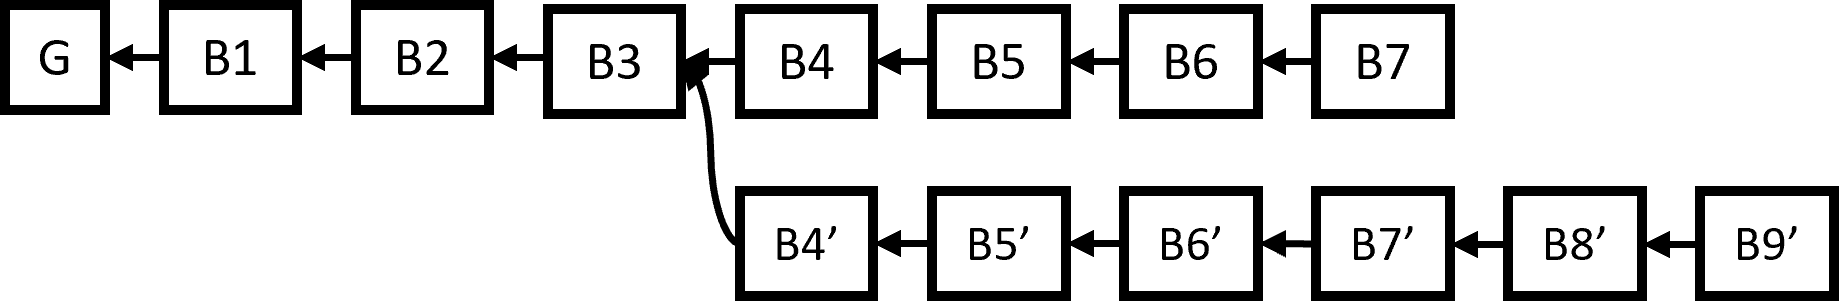
\includegraphics[width=.9\linewidth]{\FIGDIR/fork.png}
    \caption{A typical fork}
    \label{fig:fork}
\end{figure}

With operations defined as above, we will be sure that \hl{The chain in the memory pool will never get shorter}. The property is critical for the correctness of our program.

\subsection{Broadcast a transaction}
% As for broadcasting a transaction, the miner firstly will create several threads. Then, to broadcast its clients, it distributes every client with a thread and delivers the transaction to the client by gRPC through its corresponding thread.

Transaction is sent to a miner's peers through gRPC connections. Since we support a arbitrary network topology, which is \textcolor{red}{THE SECOND OPTIMIZATION}, a miner may not have connection with all the other miners in the network.

Let's say Alice want to send a transaction through gRPC connection to Bob. In the context of gRPC, Alice is the client and Bob is the server. Alice will call Bob's function to send the transaction to Bob.

How will Bob relay the transaction? If he simply send the transaction to all its peers, then we'll find that the transaction will be sent for infinite times and occupy too much network resources, or even take over all network bandwidth. The solution is \textbf{flooding alogirhtm}, i.e., Bob will first check whether he has already received the transaction(and the validity of the transaction), and then send it to its peers. This algorithm will ensure that for each transaction, every node in the network will only broadcast it once, thus utilizing limited network resources.

Actually, Bob only has to call the \textbf{Append new transacction} interface of memory pool to see whether the transaction needs to be relayed. Therefore, flooding algorithm is naturally compatible with our original design.

\subsection{Block Broadcast Session}
% We can divide block broadcast into two parts: the broadcast between the miners and the broadcast between one minor and its clients.
% \\The broadcast between the miners, which is \textcolor{red}{THE SECOND OPTIMIZATION}, supports to solve inconsistency between arbitrarily network topology. Every time when a miner adds a new block or finds a longer chain when other miner's message delivers to it, the miner needs to broadcast block to other miners. Specifically, we use binary backoff to find the common ancestor when we compare the two chains between two miners. This way is faster to find the common ancestor which generates target chains more quickly. Thus, after communication, it will reach a consensus at last.


To send a block has more issues to concern than sending a transaction. We must take inconsistency issues into consideration. Therefore, we designed \textbf{block broadcast session} based on gRPC, shown in \cref{fig:blockbroadcast}.

First, let's consider the simplest issue: There are no inconsistency issues. Suppose miner Alice creates a new block at height H+1, where H is the original height. She will broadcast it to all her peers. Each of her peers will first check the height of the block, as well as the validity of the block, and then append it to their memory pools(by calling the append block interface). The \textbf{block broadcast session} will soon finish at Stage 1. If successfully appended to the memory pool, then the block will be relayed through new \textbf{block broadcast sessions}. Each block will be broadcast by one node at most once, because 
\begin{itemize}
    \setlength{\itemsep}{1pt}
    \item When the H+1 block is added to the memory pool, memory pool will have a H+2-length chain.
    \item The memory pool will never have a shorter chain from then on as discussed in previous subsection.
    \item The H+1 height block will not pass the height check after that, so it will never be broadcast again by that node.
\end{itemize}

\begin{figure}[htbp]
    \centering
    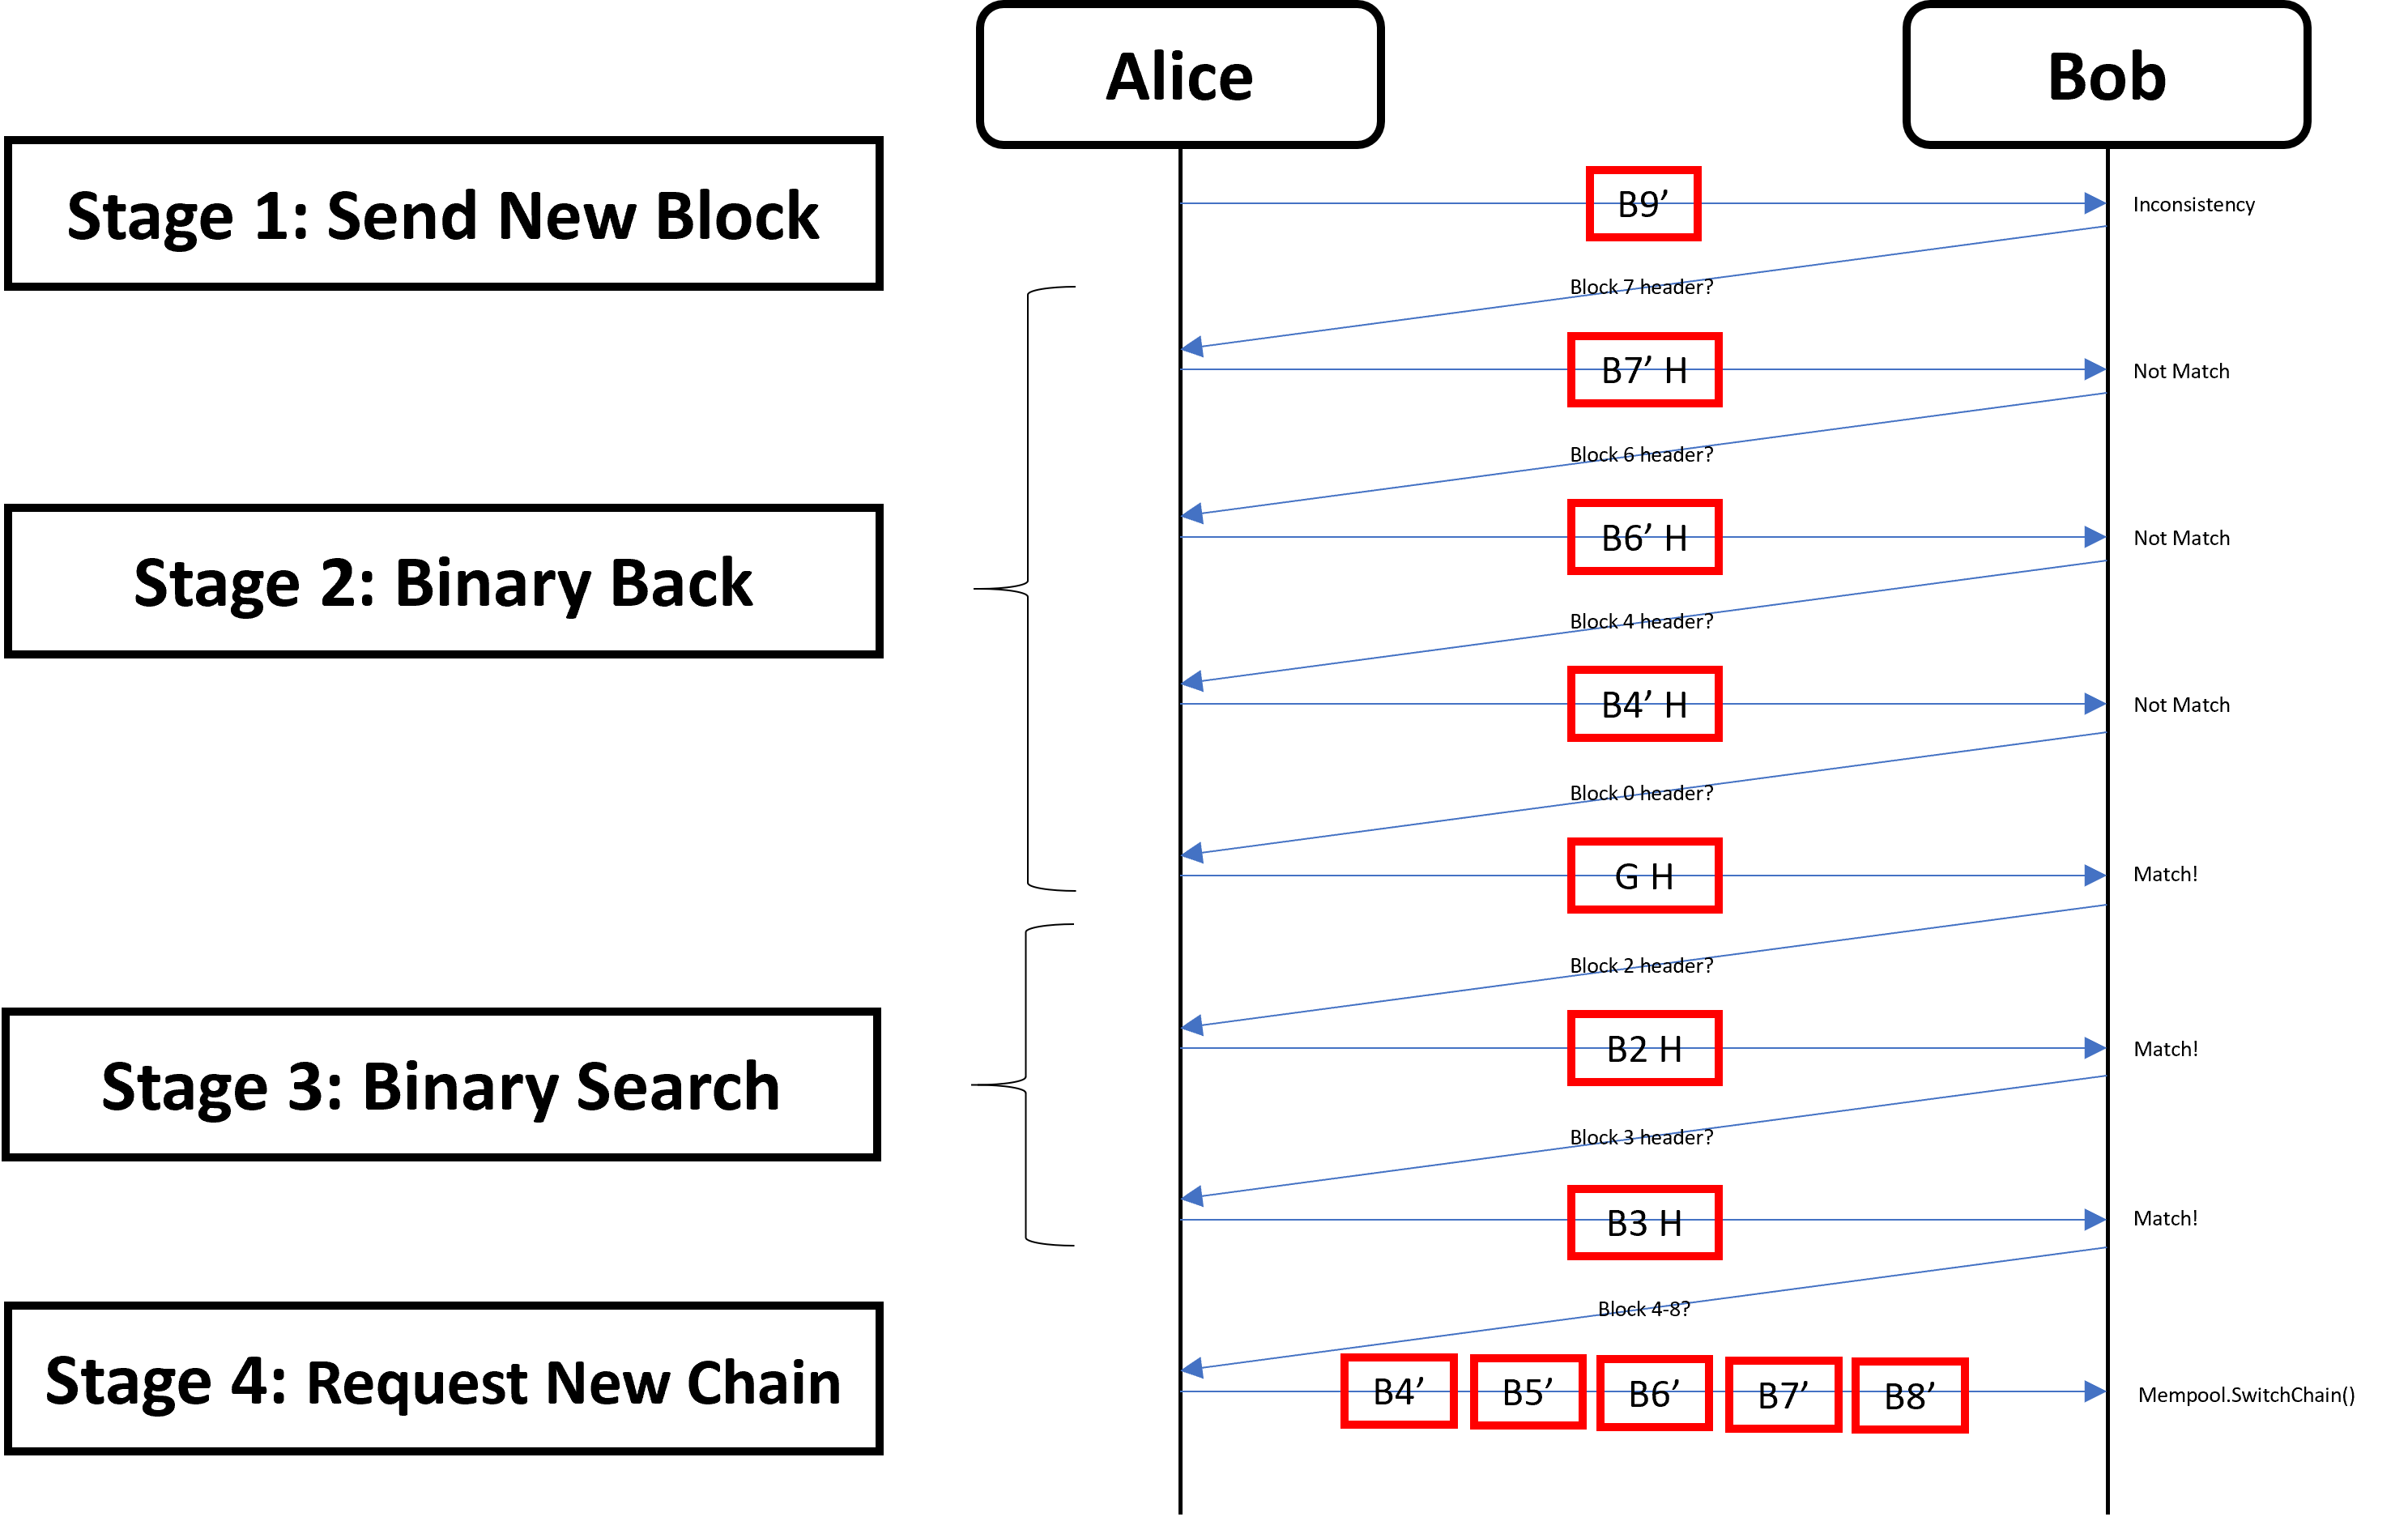
\includegraphics[width=.8\linewidth]{\FIGDIR/blockbroadcast.png}
    \caption{Broadcast Block Session}
    \label{fig:blockbroadcast}
\end{figure}

Now, let's consider when inconsistency happens. Suppose that the situation is \cref{fig:fork}. Alice now creates B9' appended to B8' and Bob has the chain ending with B7. Our session will solve the inconsistency issue as shown in \cref{fig:blockbroadcast}. 
\begin{itemize}
    \setlength{\itemsep}{1pt}
    \item In the first stage, Alice send Block B9' to Bob, and Bob will find there is an inconsistency issue.
    \item In the second stage, Bob will use binary back algorithm to find a range where inconsistency starts. The algorithm is \textcolor{red}{THE THIRD OPTIMIZATION}. Bob will finally make sure that the inconsistency starts between Block 1 to Block 4. At this stage, Bob will only request block headers, so that network resources are saved for transactions.
    \item In the third stage, Bob will use binary search algorithm to find exactly where inconsistency starts. In this situation, Bob will find that Block 4 is the first inconsistent block. 
    \item In the fourth stage, Bob will request Block 4 to Block 8 from Alice in parallel. After that, Bob will call the memory pool's Switch to a new chain interface. The memory pool will check whether the new chain is valid, and then substitute the new one for the old one. If the substitution is successful, Bob will further initiate a \textbf{block broadcast session} with his peers to broadcast the new Block 9.
\end{itemize}

A further remark on Binary Back algorithm: Actually, we can directly use binary search algorithm to find the latest inconsistent position. But it seems that at most cases, the inconsistency position is very close to the latest block, so we believe that Binary Back combined with binary search will perform better than pure binary search at most cases. 

Also notice that we only transfer headers during the second and the third stage. We believe that it will save network resources.

\section{How Client Works?}

In this section, we introduce how client process works. The client provides a user interface that a user can manage his public key addresses and billings, pay other addresses and so on. It is critical for the transaction to be put into practical use. The following \cref{fig:client} gives an overview how we implemented the client.

\begin{figure}[htbp]
    \centering
    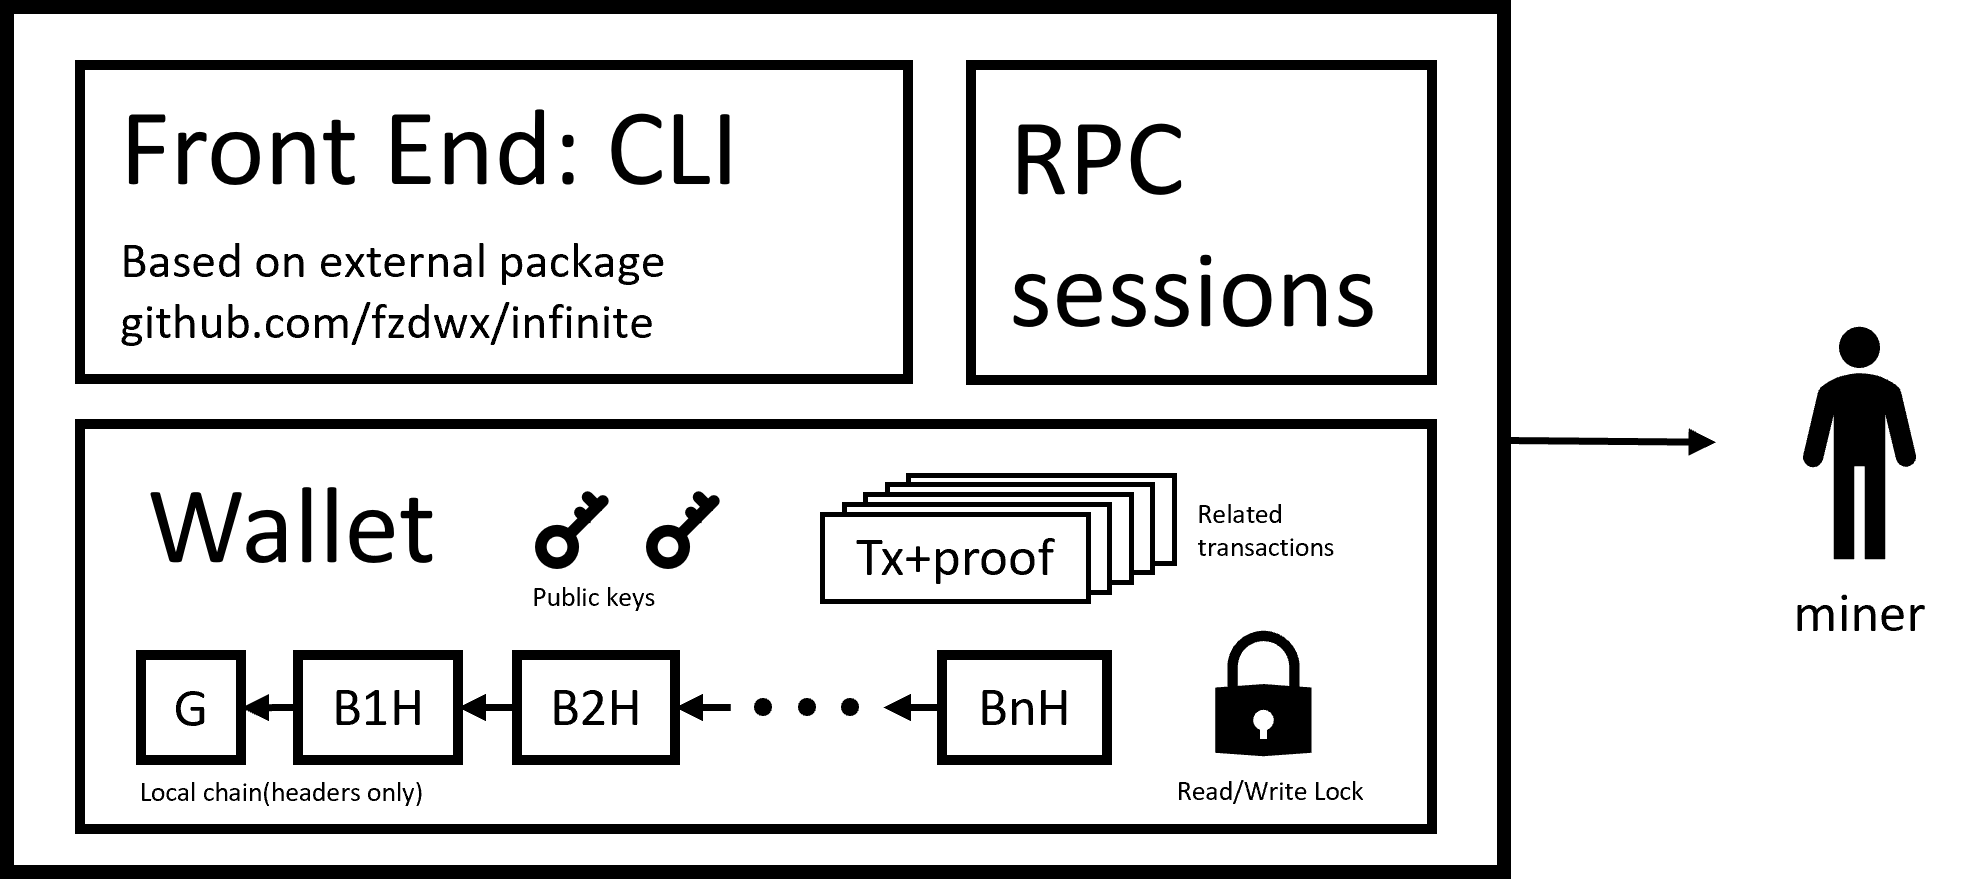
\includegraphics[width=.6\linewidth]{\FIGDIR/client.png}
    \caption{Client process}
    \label{fig:client}
\end{figure}

The client has to establish an gRPC connection with exactly one miner process. Here we make an assumption that the miner will be honest and will not lose connection. Therefore, we only have to deal with connections with only one peer for simplicity.

\subsection{Wallet}

Wallet is a abstract data structure similar to memory pool in miner process. In a wallet, we will keep 
\begin{itemize}
    \setlength\itemsep{1pt}
    \item Client's keys, i.e., public/private key pairs
    \item A chain of block headers
    \item A list of transactions as well as the merkle proof of which block the transaction is in
\end{itemize}

Also, a read/write lock is necessary for solving concurrency issues. We will not talk about the operations supported by wallet because it's not the key to client process. We only keep transactions that relate to the keys of the wallet. Therefore, we implements a \textbf{light-weight} client, without storing the whole chain of blocks and their transactions. This is our \textcolor{red}{FOURTH OPTIMIZATION}. Since we made the assumption that the miner it connects to is honest, we will always be sure that the data in the wallet is correct.

For storing all related transactions, we used database implemented by package \url{github.com/go-gota/gota}. It helped us with easier filter and selection operations.

\subsection{Command Line Interface}

We implemented a CLI based on package \url{github.com/fzdwx/infinite}. The CLI is really easy to use, which is our \textcolor{red}{FIFTH OPTIMIZATION}. To be conclusive, it supports the following operations:
\begin{itemize}
    \setlength{\itemsep}{1pt}
    \item Creates a public key address
    \item Save an already-known public key address
    \item Construct and broadcast a transaction
    \item View transactions according to time range and public key address
\end{itemize}
Follow the instructions given by CLI and you will learn how to do the above things without any documentation!

\section{Future Work}

There are still much improvement that can be made to current project. We mentioned in the second section that the current transaction system doesn't support contracts. We can add to contract support in the future, so that the transaction system can express more financial meanings. The current communication system, based on gRPC, might not be extensible. Currently, we have tested a 5-miner system with different topologies and more tests can be done in the future. We could also focus on a better incentive mechanism. The current version will mint 1024 coins for each block and the difficulty of proof-of-work puzzle never changes, which will lead to corruption of the financial system. User interface may also be updated, with more functionalities or even a graphical interface.

\bibliographystyle{IEEEtran}
\bibliography{ref}

\end{spacing}
\end{document}

%%%%%%%%%%%%%%%%%%%%%%%%%%%%%%%%%%%%%%%%%%%%%%%%%%%%%%%%%%%%%

